\documentclass[11pt]{article}
\renewcommand{\baselinestretch}{1.05}
\usepackage{amsmath,amsthm,verbatim,amssymb,amsfonts,amscd, graphicx}
\usepackage{blindtext}

\usepackage{caption}
\usepackage{enumitem}

%Additional Packages
\usepackage{enumitem}
\usepackage{graphics}
\usepackage{float}
\graphicspath{ {images/} }
%\usepackage[framed]{mcode}
\usepackage{hyperref}
\hypersetup{
	colorlinks=true,
	linkcolor=blue,
	filecolor=magenta,      
	urlcolor=cyan,
}

\topmargin0.0cm
\headheight0.0cm
\headsep0.0cm
\oddsidemargin0.0cm
\textheight23.0cm
\textwidth16.5cm
\footskip1.0cm
\theoremstyle{plain}
\newtheorem{theorem}{Theorem}
\newtheorem{corollary}{Corollary}
\newtheorem{lemma}{Lemma}
\newtheorem{proposition}{Proposition}
\newtheorem*{surfacecor}{Corollary 1}
\newtheorem{conjecture}{Conjecture} 
\newtheorem{question}{Question} 
\theoremstyle{definition}
\newtheorem{definition}{Definition}

\usepackage{indentfirst}
%\renewcommand{\thesubsubsection}{\thesubsection.\alph{subsection}}

\newcommand{\floor}[1]{\lfloor #1 \rfloor}

%SETUP PSUEDOCODE
\usepackage{tcolorbox}


%SETUP AtxMEGA128A1U
\usepackage{listings}

\usepackage{xcolor}
\definecolor{bluekeywords}{rgb}{0.13,0.13,1}
\definecolor{greencomments}{rgb}{0,0.5,0}
\definecolor{turqusnumbers}{rgb}{0.17,0.57,0.69}
\definecolor{redstrings}{rgb}{0.5,0,0}

\lstdefinelanguage{atxmega128a1u}{
	morekeywords={include, ,org, rjmp, CSEG, db, equ, DSEG, match, with, rec, open, module, namespace, type, of, member, and, for, in, do, begin, end, fun, function, try, mutable, if, then, else},
	keywordstyle=\color{bluekeywords},
	sensitive=false,
	morecomment=[l][\color{greencomments}]{;},
	morecomment=[s][\color{greencomments}]{{/*}{*/}},
	morestring=[b]",
	stringstyle=\color{redstrings}
}

\lstnewenvironment{asmlisting}{
	\lstset{
		frame=single,
		language=atxmega128a1u,
		basicstyle=\ttfamily,
		breaklines=true,
		columns=fullflexible
	}
}
{}



\begin{document}
\captionsetup[figure]{labelfont=bf} 

\title{Lab 0}
\author{\textbf{Michael Arboleda}\\Lab Section: 7F34}
\maketitle
\section*{b. Answers to all pre-lab questions}
\begin{enumerate}[label={\arabic*)},font={\color{red}\bfseries}]
	%
	%1
	%
	\item \textbf{What minimum lab average is required in order to be eligible to pass the course?}\\[0.8ex]
	\textbf{ANS:} 65\%
	%
	%2
	%
	\item \textbf{Can you drop this lab if ... a) you overslept? b) project for other class due?}\\[0.8ex]
	\textbf{ANS:} Yes, Yes
	%
	%3
	%
	\item \textbf{How late can you arrive for lab and still be admitted? How late can you arrive for lab and still be allowed to take the lab quiz?}\\[0.8ex]
	\textbf{ANS:} You can be up to 30 minutes late and still be admitted. You can be up to 10 minutes late and still take the quiz. 
	%
	%4
	%
	\item \textbf{What is the lab makeup policy if you miss a single lab?}\\[0.8ex]
	\textbf{Ans:} If you miss a single-lab, you cannot make it up\\
	%
	%5
	%
	\item \textbf{When soldering a wire to a pin, what should the soldering iron touch and what should the un-melted solder touch? }\\[0.8ex]
	\textbf{ANS:} The soldering iron should touch the pin. The un-melted solder should touch the wire. 
	%
	%6
	%
	\item \textbf{What instruction can be used to read from program memory (flash)? Can you use any registers with this instruction?}\\[0.8ex]
	\textbf{ANS:} LPM (and ELPM for extended address) is used to read from program memory. You cannot use any register, you must use the Z register
	%
	%7
	%
	\item \textbf{What are the key differences between program and data memory? See section 7 in the ATxmega128A1U manual}\\[0.8ex]
	\textbf{ANS:} Program memory can hold executable code. Data Memory cannot hold executable code. Data memory also includes the internal SRAM and EEPROM for nonvolatile data storage.
	%
	%8
	%
	\item \textbf{When using RAM (not EEPROM), what memory locations can be utilized for the .DSEG? Why? What .DSEG did you use in this lab and why?}\\[0.8ex]
	\textbf{ANS:} Memory address 0x2000 and above are for the ram. This is because 0x1000 to 0x1FFF is the EEPROM. The .DESG used in the lab is 0x3744. This was because it was in the directions of the lab document.
	
	 
	
\end{enumerate}
\section*{c. Problems Encountered}
At first I did not understand the data reading. This was clarified in lecture when Dr. Schwartz went over the CPU\textunderscore RAMPZ register
\section*{d. Future Work/Applications}
After doing this lab there is clearly so much to learn. There are many other instructions I could have used instead of the ones I used. I could try using those instructions instead so I can understand them and not be stuck knowing only a small subset of all the commands
\section*{e. Schematics}
N/A (No hardware to change)
\section*{g. Pseudocode/Flowcharts}
\textbf{\textcolor{blue}{Pseudocode for lab0.asm:}}
\begin{tcolorbox}
\begin{verbatim}
* Create array pointer 
* Create pointer for storing

DO-LOOP
    * Get Data From Array
    * Increment array pointer 

    IF(DATA LESS THAN 166){
        IF(DATA GRATER THAN 36){
            * Add data and 0x11
        }
        * Store value
    }
WHILE(DATA is not 0)

\end{verbatim}
\end{tcolorbox}
\section*{h. Program Code}
\lstinputlisting[language=atxmega128a1u, frame=single]{lab0c.asm}
\section*{i. Appendix}
\begin{figure}[H]
	\centering
	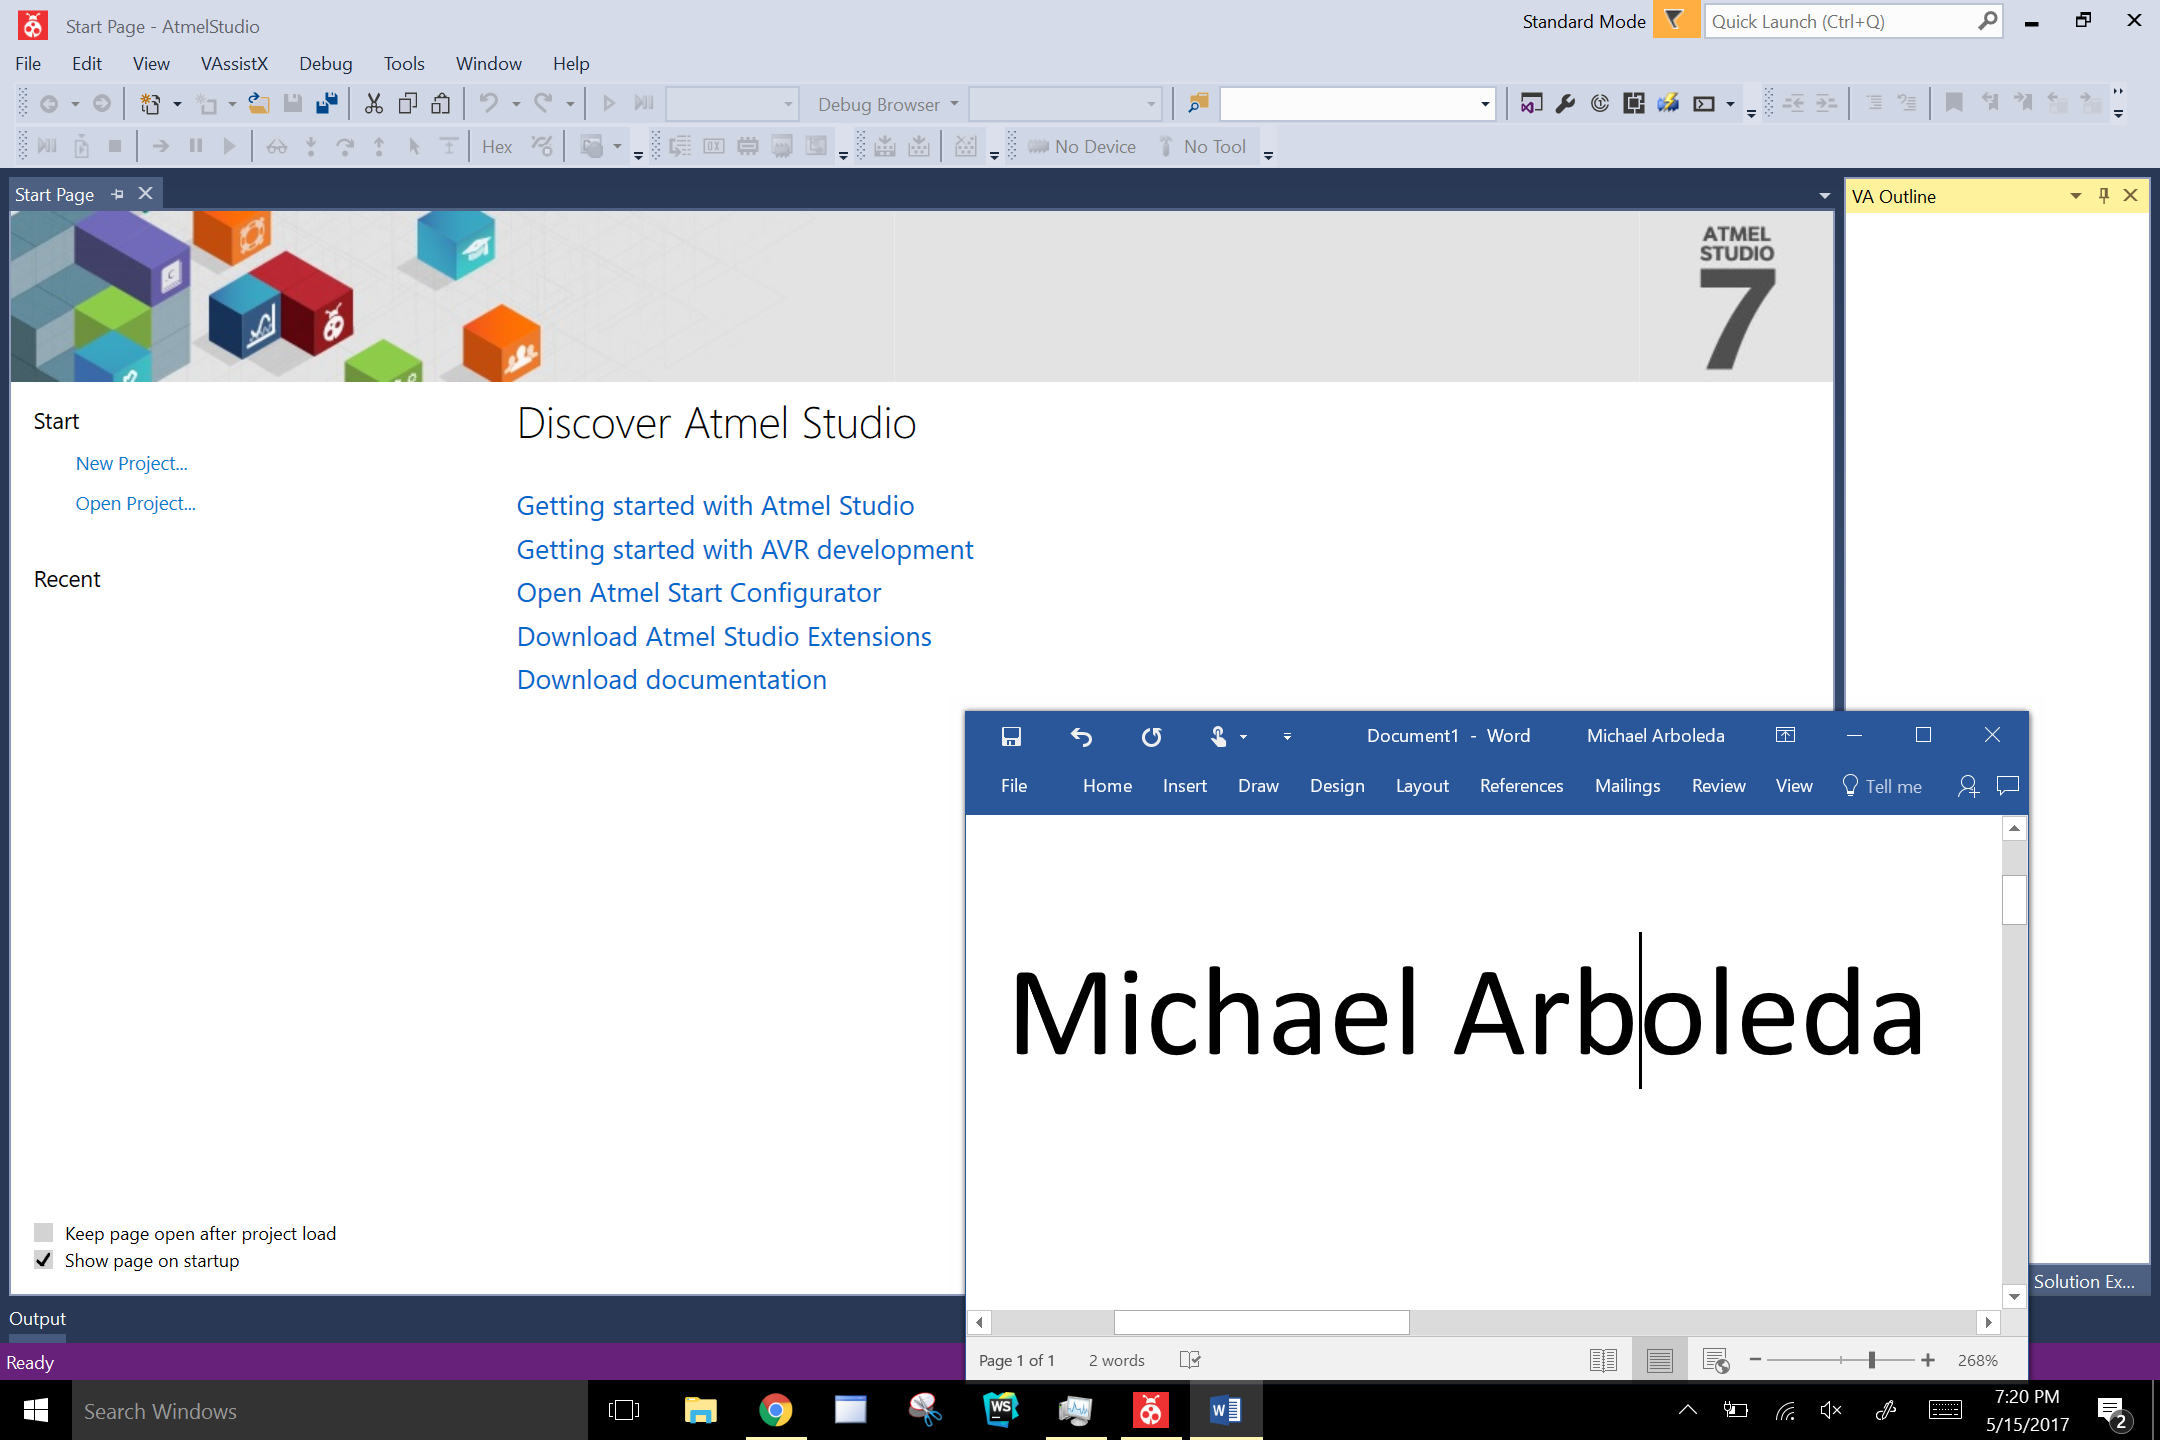
\includegraphics[width=\textwidth]{prelabA}
	\label{fig:PLA}
	\caption{PART A. ATMEL Installation}
\end{figure}

\begin{figure}[H]
	\centering
	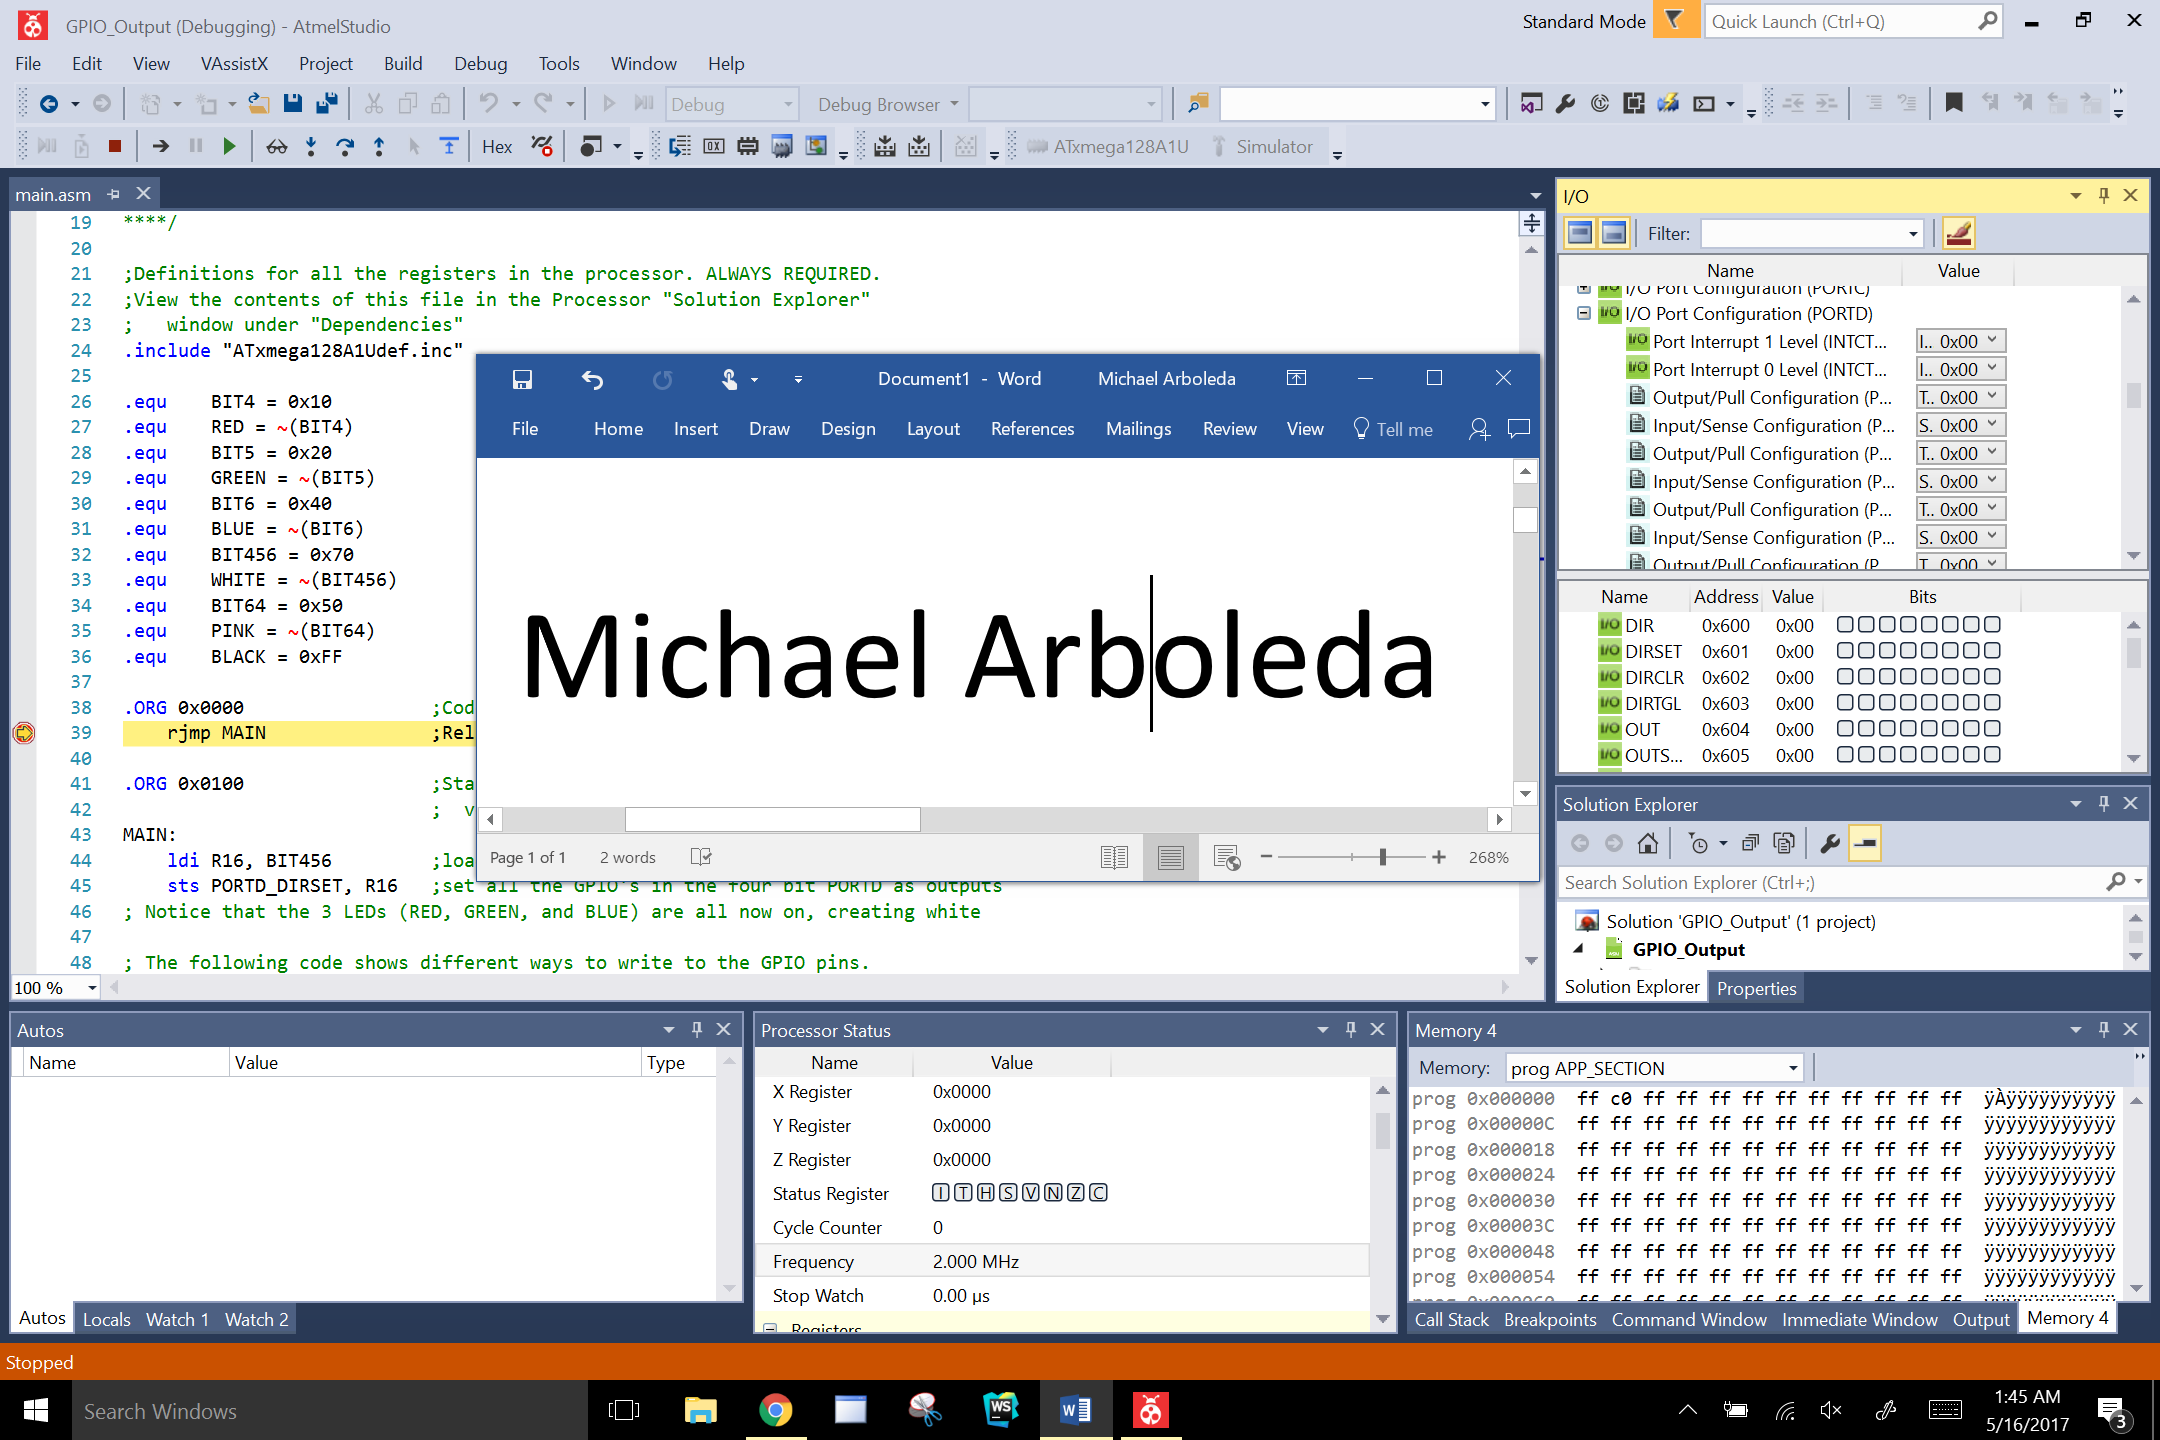
\includegraphics[width=\textwidth]{prelabB}
	\label{fig:PLB}
	\caption{PART B. ATMEL Tutorial}
\end{figure}

\end{document}